\label{sec:5.3}

%%%%%%%%%%%%%%%%%%%%%%%%%%%%%%%%%%%%%%%%%%%%%%%%%%%%%%%
%(Prakash) Discuss ADC Core linearity
%%%%%%%%%%%%%%%%%%%%%%%%%%%%%%%%%%%%%%%%%%%%%%%%%%%%%%%

Measured ADC INL is approximately 1 LSB at 12-bit level, however simulations suggest 0.5 LSB INL is possible. The main drawback is lack of corner models at cold and the the Monte Carlo analysis at warm was insufficient.

%We investigated two main suspects: Incomplete reference (and/or threshold) settling and Large closed-loop gain non-linearity in the stages.

%When the calibration signal is applied the threshold references receives a big kick. This was simulated (figure \ref{fig:ref_settling}) to ensure settling was adequate, but this could be the problem.

%\begin{figure}[h!]
%\centering
%  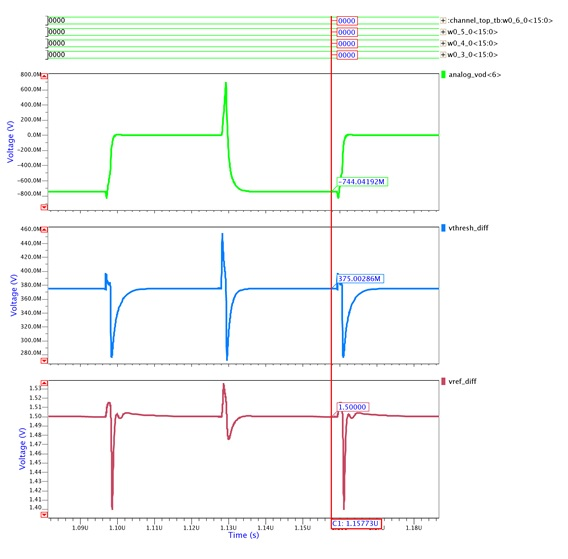
\includegraphics[width=0.7\linewidth]{figures/prakash_fig/ref_settling.JPG}
%  \caption{ADC reference settling}
%  \label{fig:ref_settling}
%\end{figure}

%Reference settling issue was investigated by increasing the current of the reference buffers, on the other hand the reference buffers themselves may also be struggling to settle. This was investigated by slowing down the chip. 

The ADC linearity is limited by insufficient op-amp gain in the stages. Since the calibration algorithm can only correct linear gain errors, non-linearity beyond the expectation could and will limit the performance. The op-amp becomes nonlinear as their swing increases because the output resistance of the devices connected to the output decreases when the voltage across them is reduced. The main suspect is the raw open-loop gain is lower than expected and the closed-loop rejection of the non-linearity is not good enough. To verify the large closed-loop gain non-linearity in the stages, 
%references were clamped down and the evidence of op-amps becoming less and less non-linear when we reduce the swing become apparent. 
reference voltages were adjusted to reduce the dynamic range of each stage and measurements demonstrate that this increased the linearity.
Figures \ref{fig:linearity_100mv} through \ref{fig:linearity_300mv} demonstrate this. 

%%\begin{figure}[h!]
%%\centering
%%  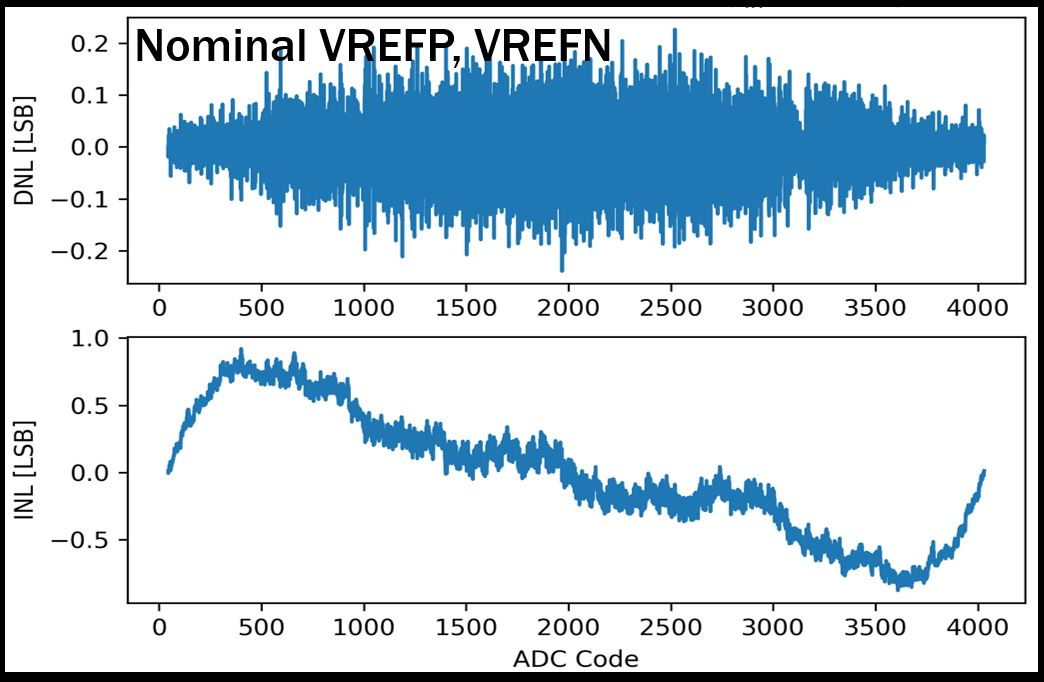
\includegraphics[width=0.5\linewidth]{figures/prakash_fig/linearity_nominal.JPG}
%%  \caption{ADC linearity with nominal VREFN/P }
%%  \label{fig:linearity_nominal}
%%\end{figure}

\begin{figure}[h!]
\centering
  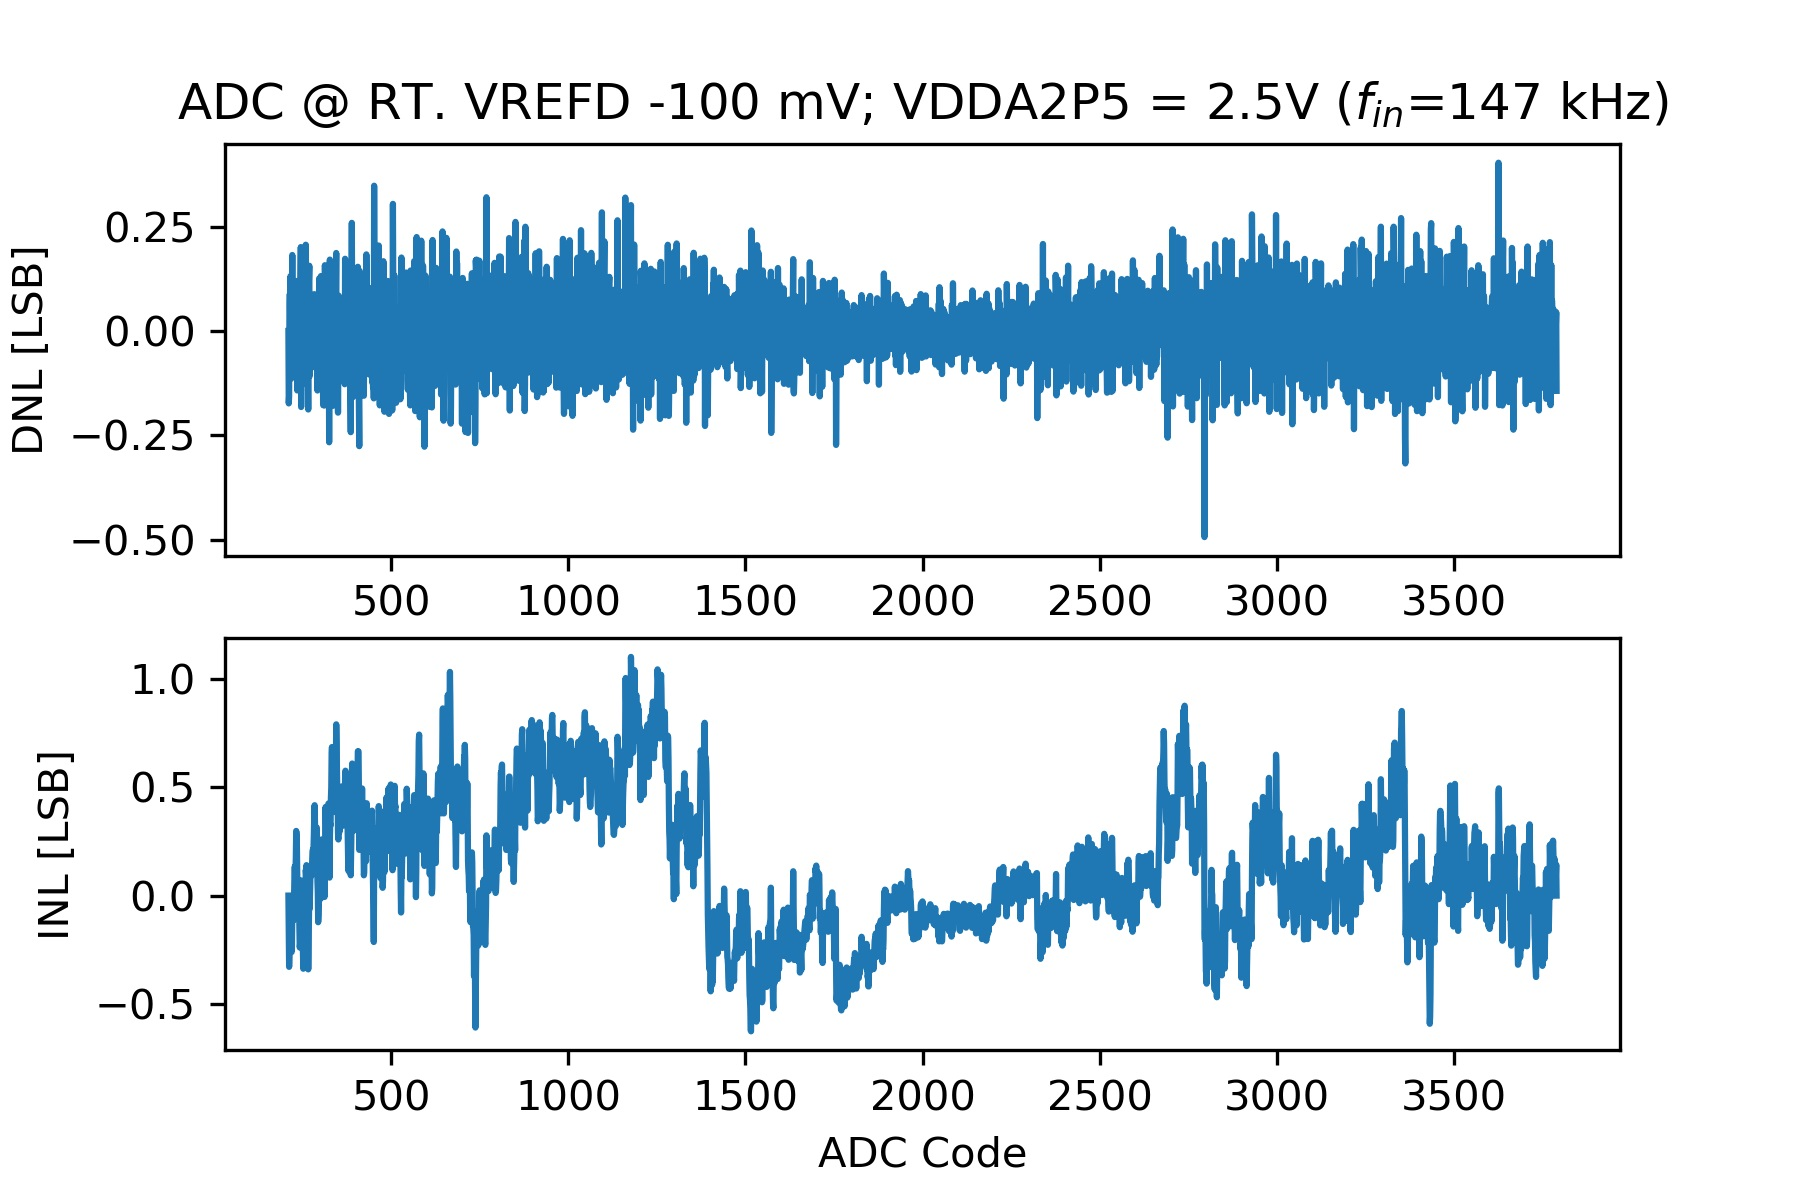
\includegraphics[width=0.7\linewidth]{figures/prakash_fig/linearity_100mv.JPG}
  \caption{ADC linearity with VREFN/P +/- 100mV}
  \label{fig:linearity_100mv}
\end{figure}

\begin{figure}[h!]
\centering
  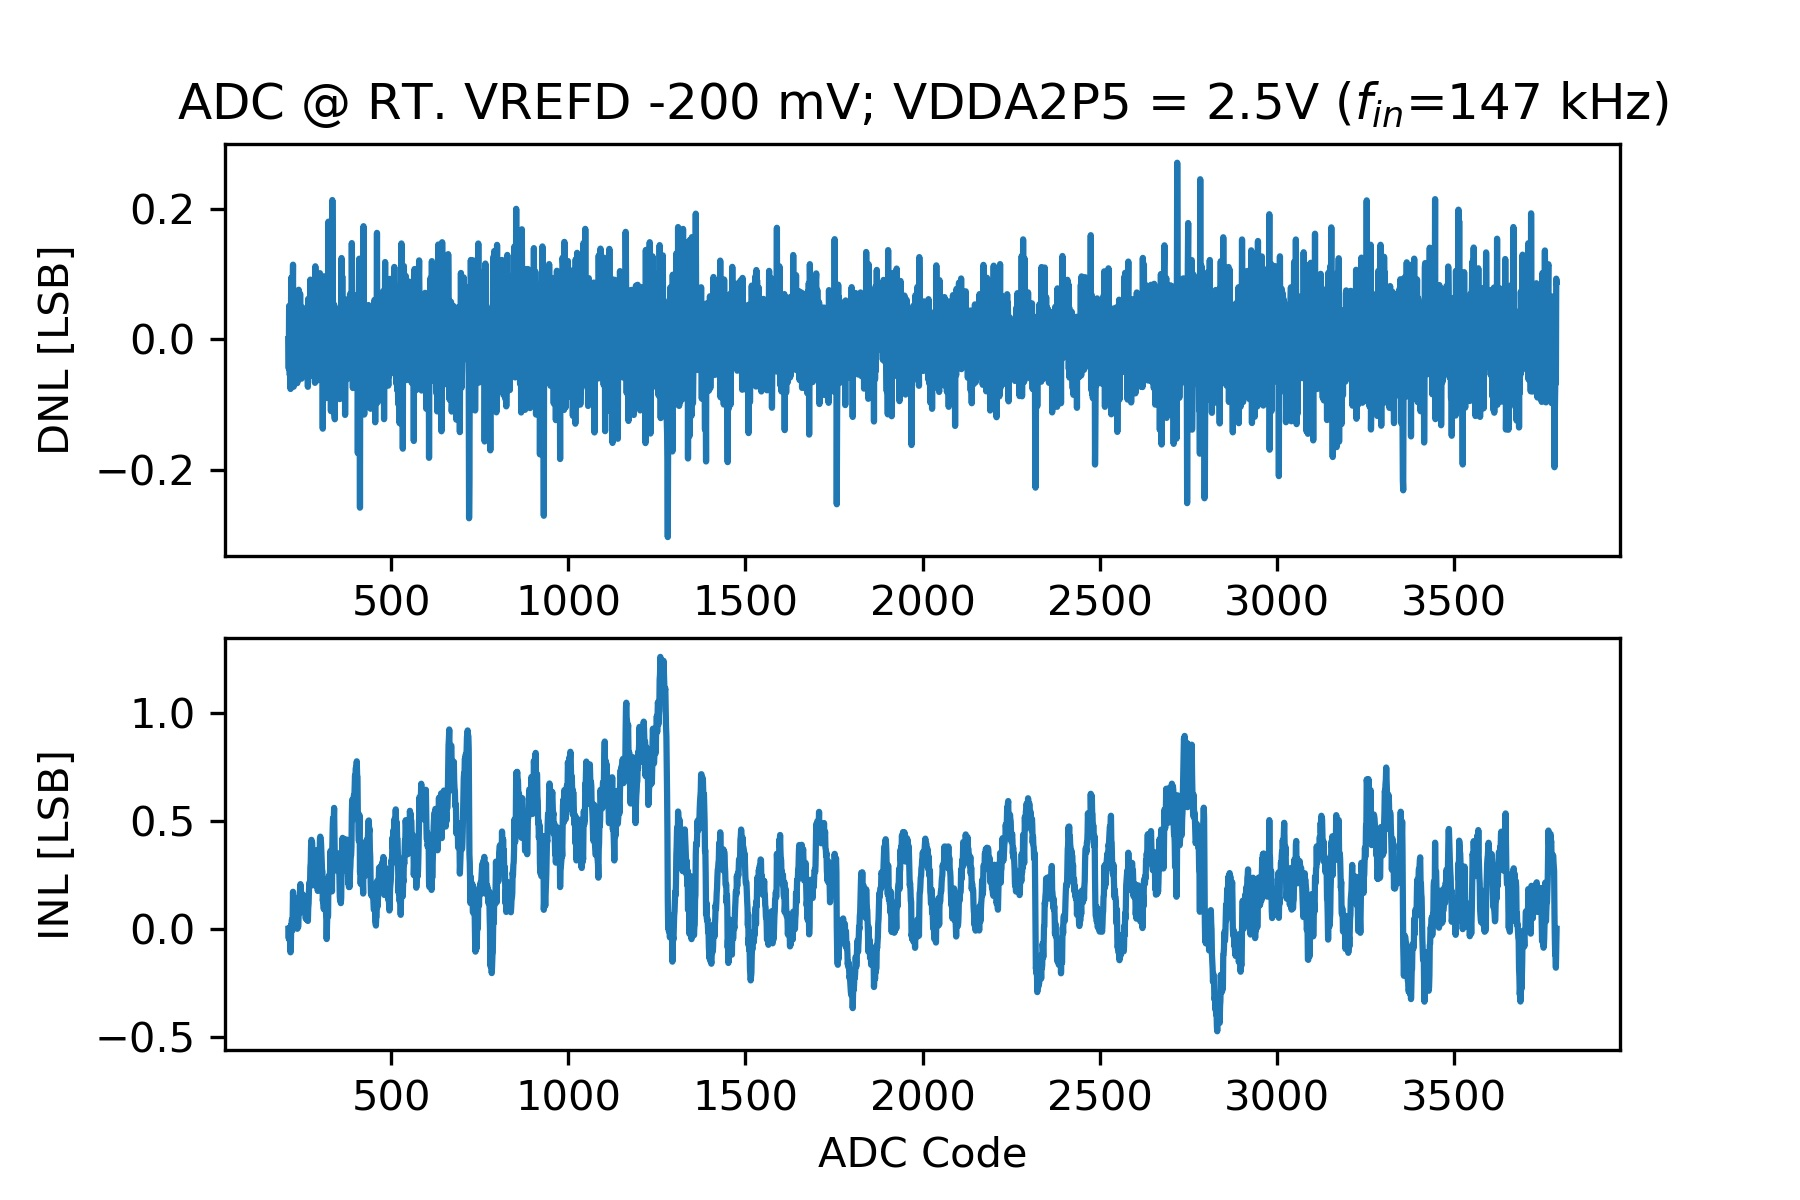
\includegraphics[width=0.7\linewidth]{figures/prakash_fig/linearity_200mv.JPG}
  \caption{ADC linearity with VREFN/P +/- 200mV}
  \label{fig:linearity_200mv}
\end{figure}

\begin{figure}[h!]
\centering
  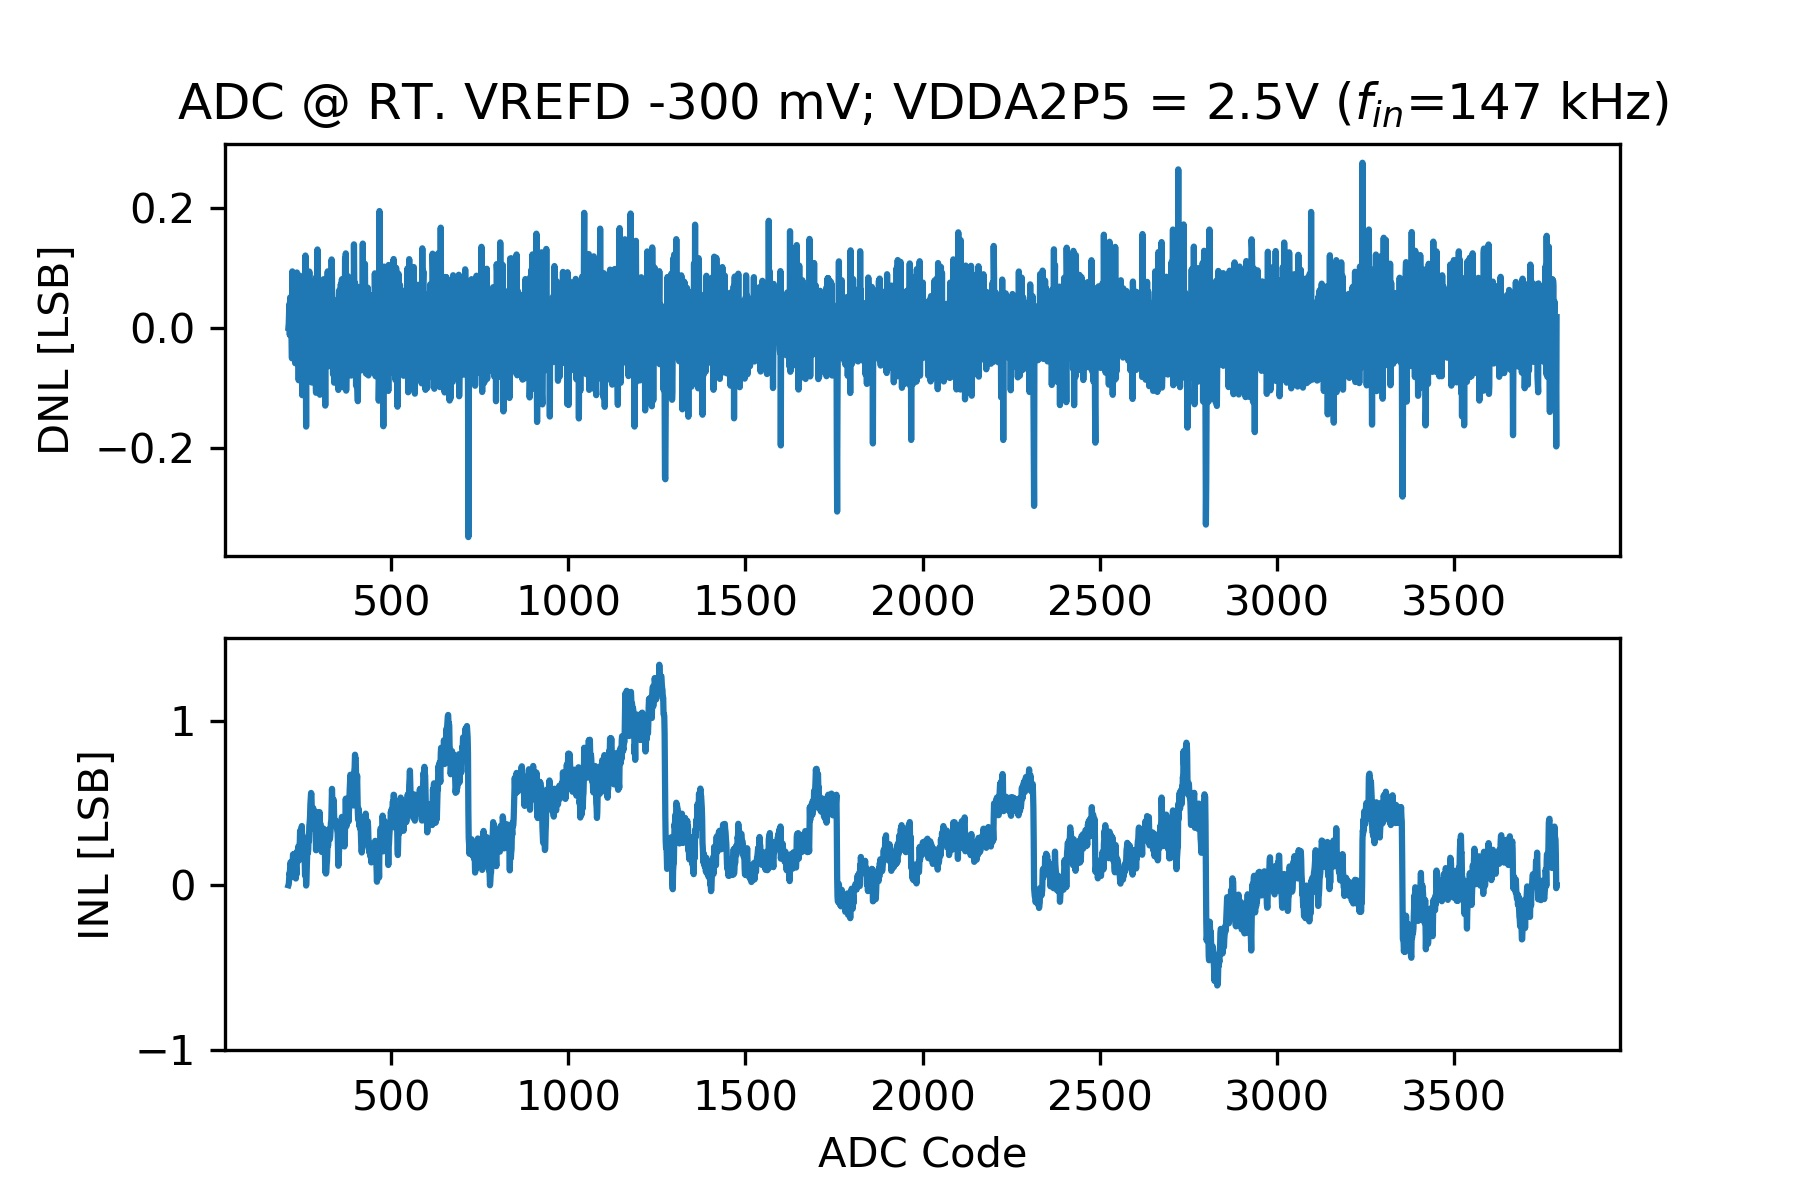
\includegraphics[width=0.7\linewidth]{figures/prakash_fig/linearity_300mv.JPG}
  \caption{ADC linearity with VREFN/P +/- 300mV}
  \label{fig:linearity_300mv}
\end{figure}

Slowing down ADC by 16X and reducing bias currents to increase op-amp gain improves linearity, while increasing bias currents at full speed doesn’t help, this is a key evidence to rule out other issues like settling issues.

The calibration algorithm is linear, and does little to improve performance in presence of non-constant stage gain. Negative feedback rejects non-linearity in the stage via high open-loop gain. In other words, high op-amp gain is needed to keep the stages linear so the calibration algorithm can work.

Each op-amp includes a gain-boosting circuit to increase the open-loop gain. The gain boosting amplifiers increase the op-amp gain by a factor of 5 in simulation. 

\begin{figure}[h!]
\centering
  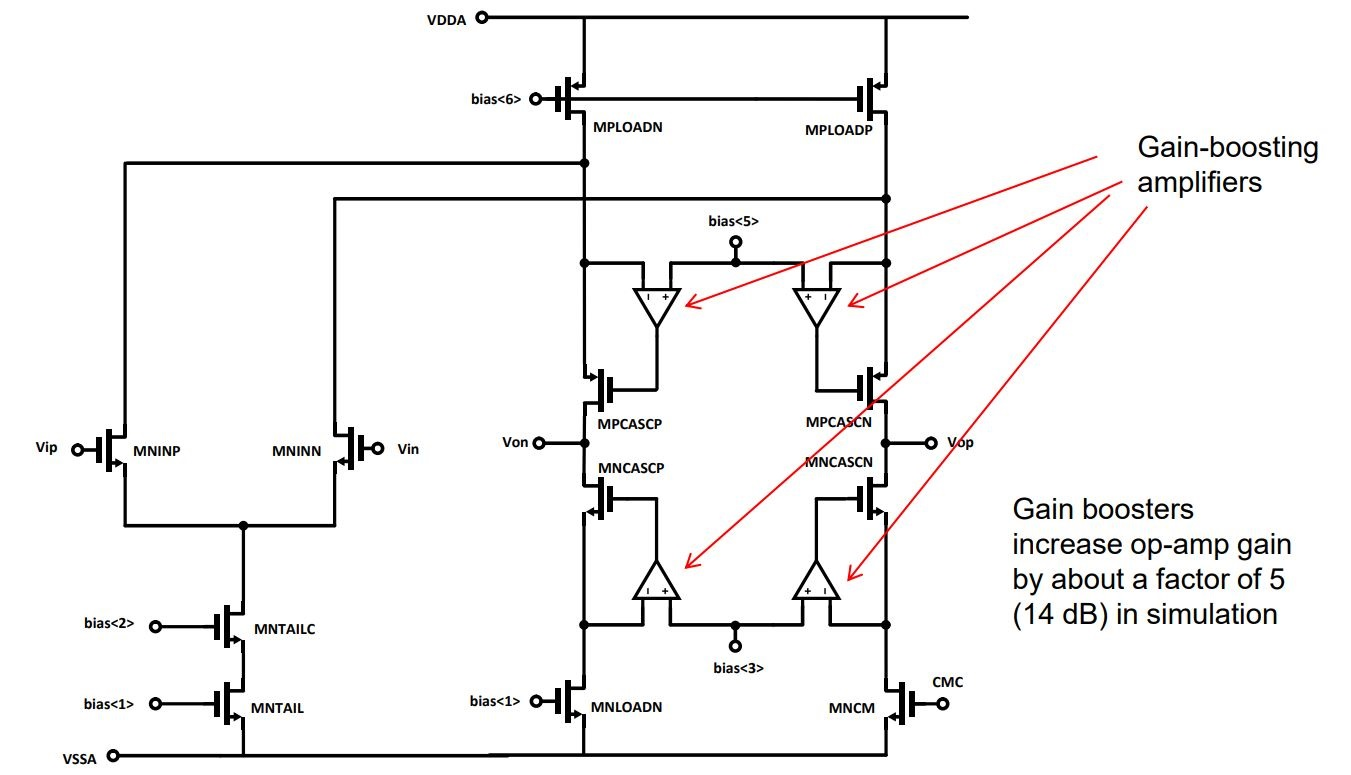
\includegraphics[width=0.9\linewidth]{figures/prakash_fig/op_amp.JPG}
  \caption{Op Amp}
  \label{fig:op_amp_1}
\end{figure}

The gain-boosters can be controlled externally by the configuration bits, figures \ref{fig:linearity_GB_ON} and \ref{fig:linearity_GB_OFF} show the measured linearity of the ADC with gain-boosters ON and OFF. All the measurements were taken by clocking the ADC at 1MHz (nominal 16MHz) and nominal reference voltages.  

\begin{figure}[h!]
\centering
  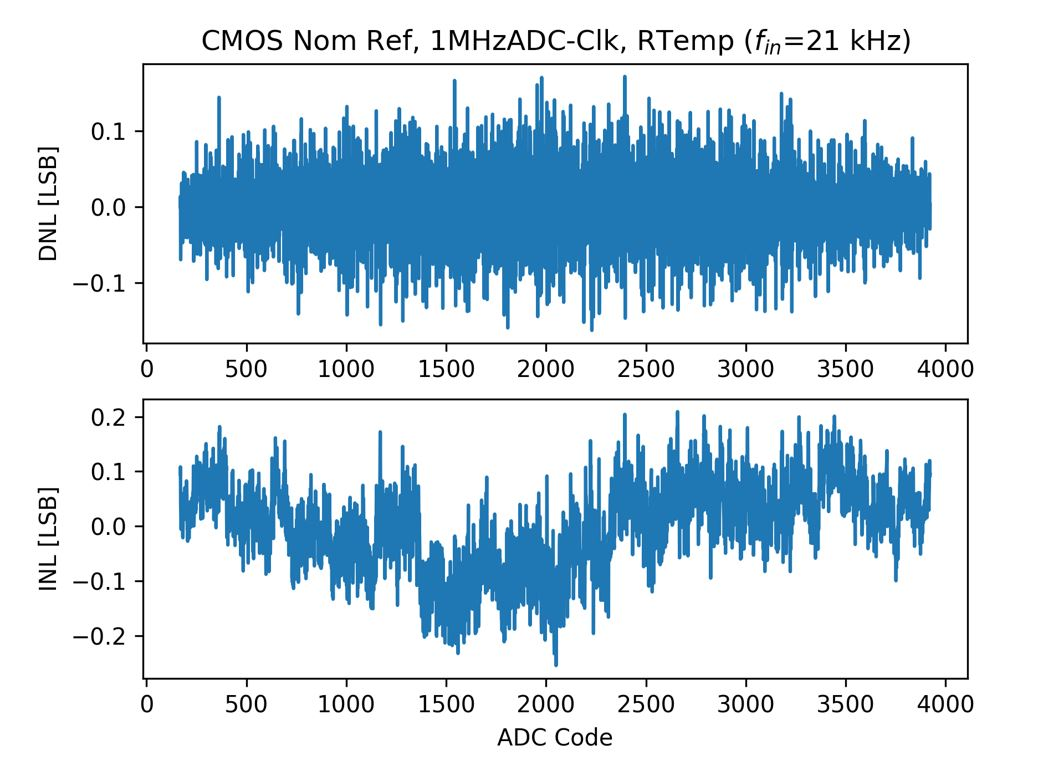
\includegraphics[width=0.6\linewidth]{figures/prakash_fig/linearity_GB_ON.JPG}
  \caption{Linearity with Gain Boosters ON}
  \label{fig:linearity_GB_ON}
\end{figure}

\begin{figure}[h!]
\centering
  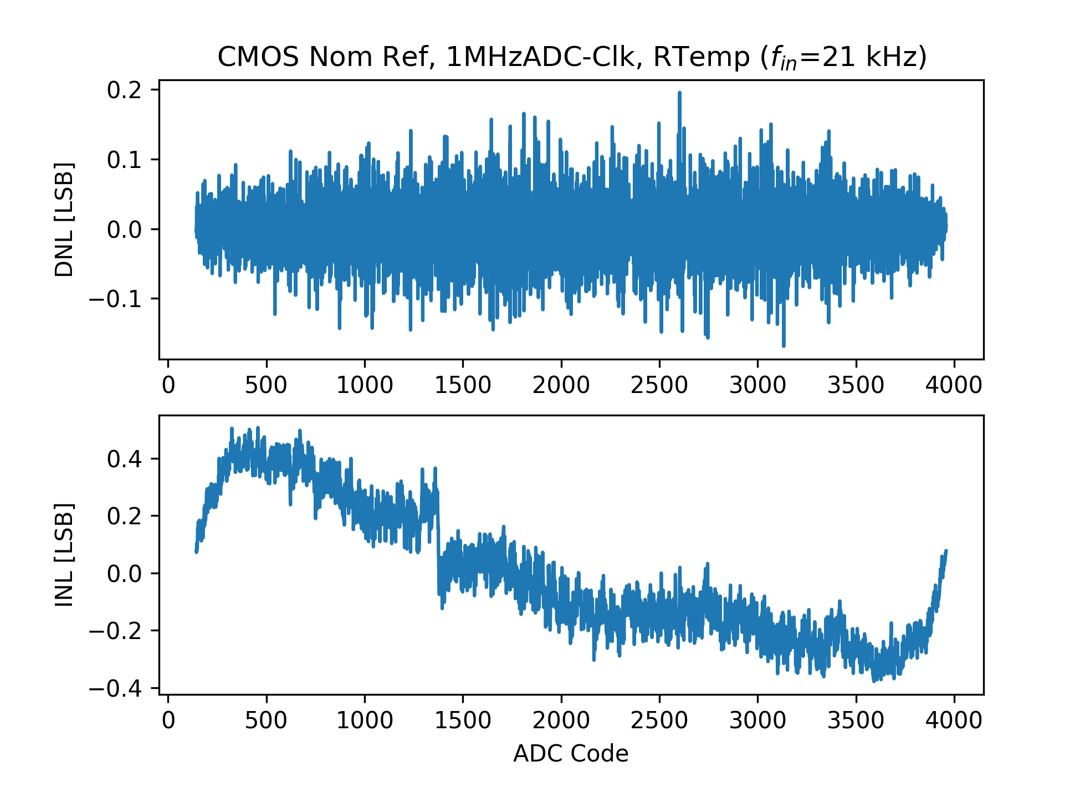
\includegraphics[width=0.6\linewidth]{figures/prakash_fig/linearity_GB_OFF.JPG}
  \caption{Linearity with Gain Boosters OFF}
  \label{fig:linearity_GB_OFF}
\end{figure}

Behavioral modeling was performed to verify the open loop gain of the op-amp with gain boosters ON and OFF. 

\begin{figure}[h!]
\centering
  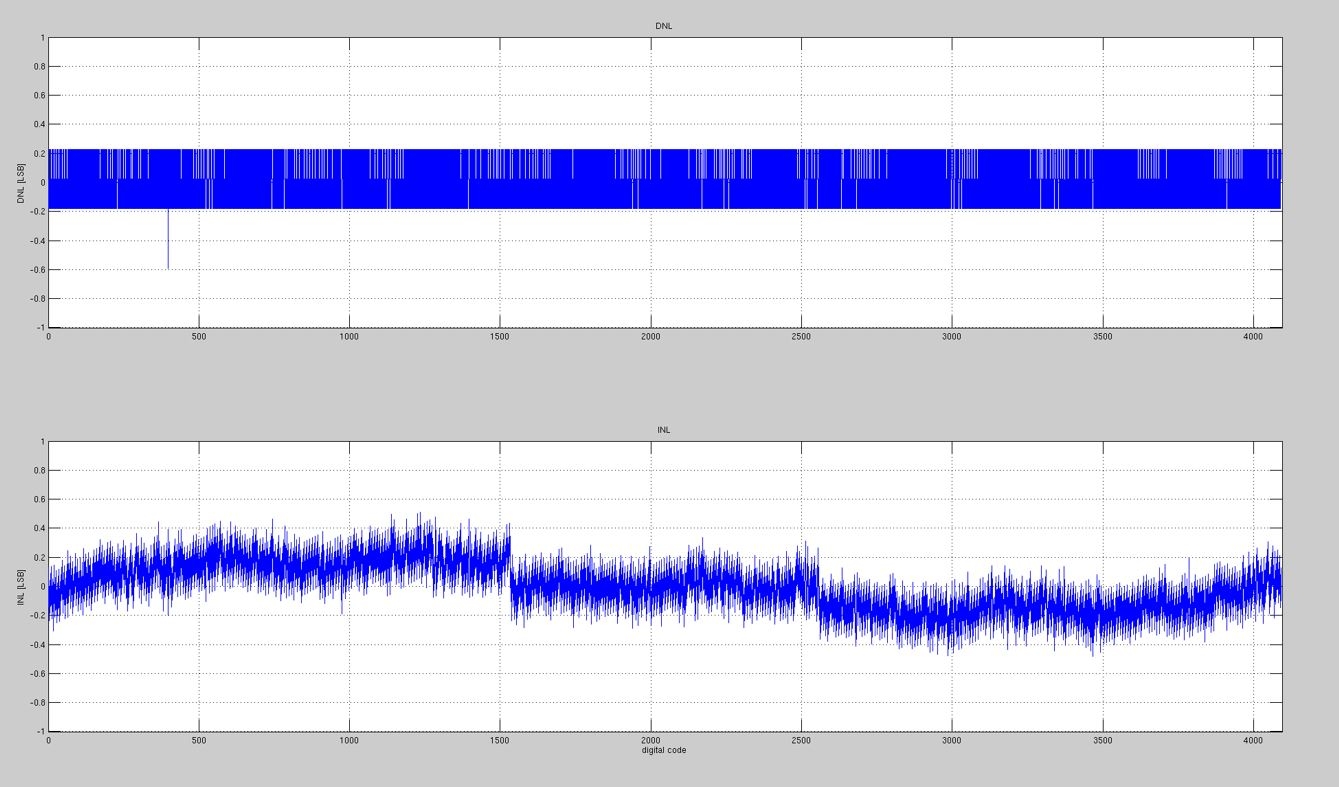
\includegraphics[width=0.6\linewidth]{figures/prakash_fig/behav_GB_ON.JPG}
  \caption{MATLAB model - gain boosters on -> 80 dB op-amp gain}
  \label{fig:behav_GB_ON}
\end{figure}

\begin{figure}[h!]
\centering
  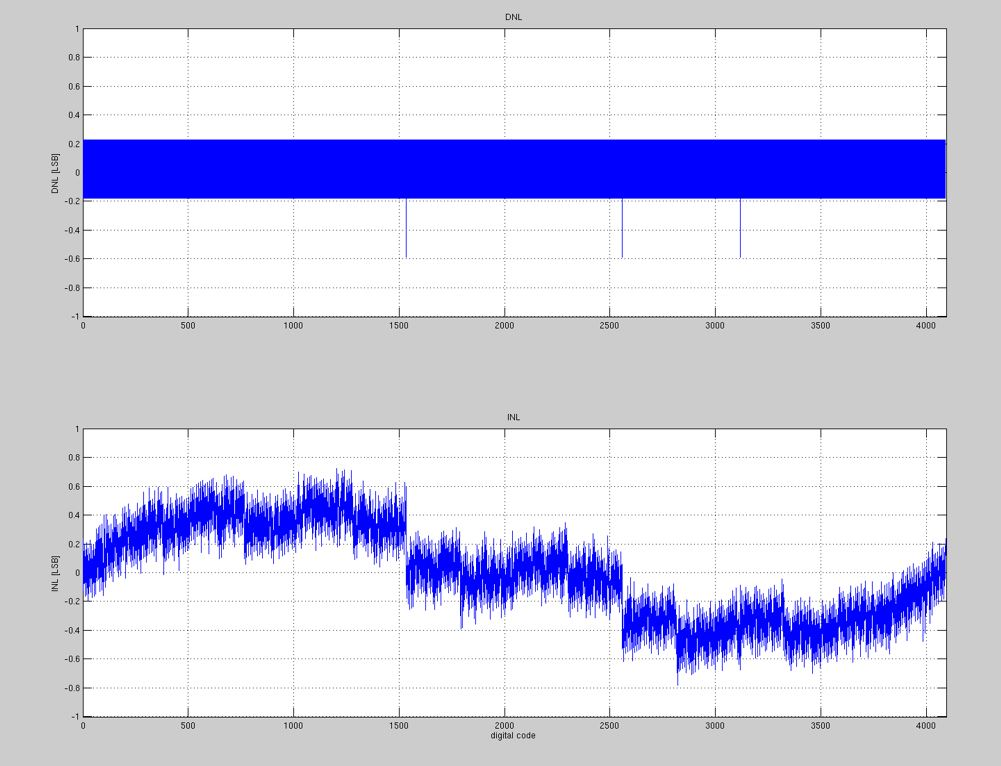
\includegraphics[width=0.6\linewidth]{figures/prakash_fig/behav_GB_OFF.JPG}
  \caption{MATLAB model - gain boosters off -> 74 dB op-amp gain}
  \label{fig:behav_GB_OFF}
\end{figure}

Figures \ref{fig:linearity_GB_ON}, \ref{fig:behav_GB_ON} and figures \ref{fig:linearity_GB_OFF}, \ref{fig:behav_GB_OFF} have roughly similar performances. The gain boosters improve the open loop gain by 6 dB instead of 14dB, i.e, the gain boosters are adding 2X gain and not 5X gain as expected. 

Analysis indicates not a lot of margin on the gain booster design for biasing. Also, the fact linearity doesn't improve at cold as much as we thought it would, also points to a biasing issue. The op-amp can be improved by centering the gain booster biasing for more margin. 

Corner analysis on the op-amp was performed to understand the issues better and the gain booster circuit was modified to improve the overall gain of the op-amp. Figures \ref{fig:opamp_gain_rt} and \ref{fig:opamp_gain_m_rt} show the corner analysis of the op-amp circuit at room temperature.

\begin{figure}[h!]
\centering
  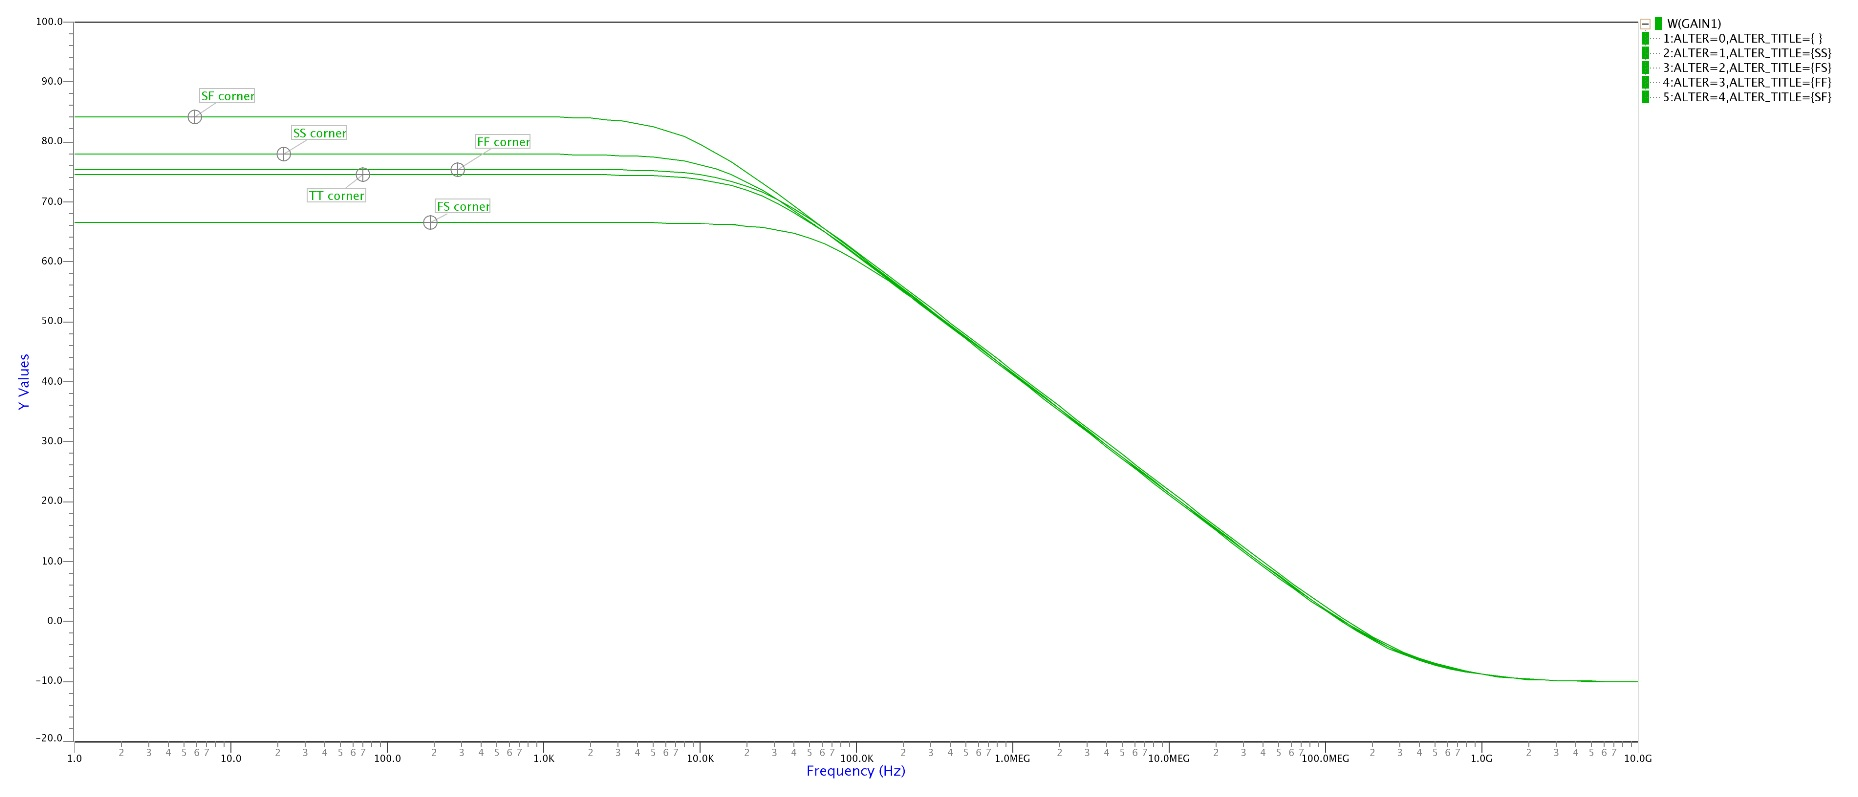
\includegraphics[width=0.8\linewidth]{figures/prakash_fig/opamp_gain_rt.JPG}
  \caption{Corner analysis of the op-amp gain, with current gain booster circuit}
  \label{fig:opamp_gain_rt}
\end{figure}

\begin{figure}[h!]
\centering
  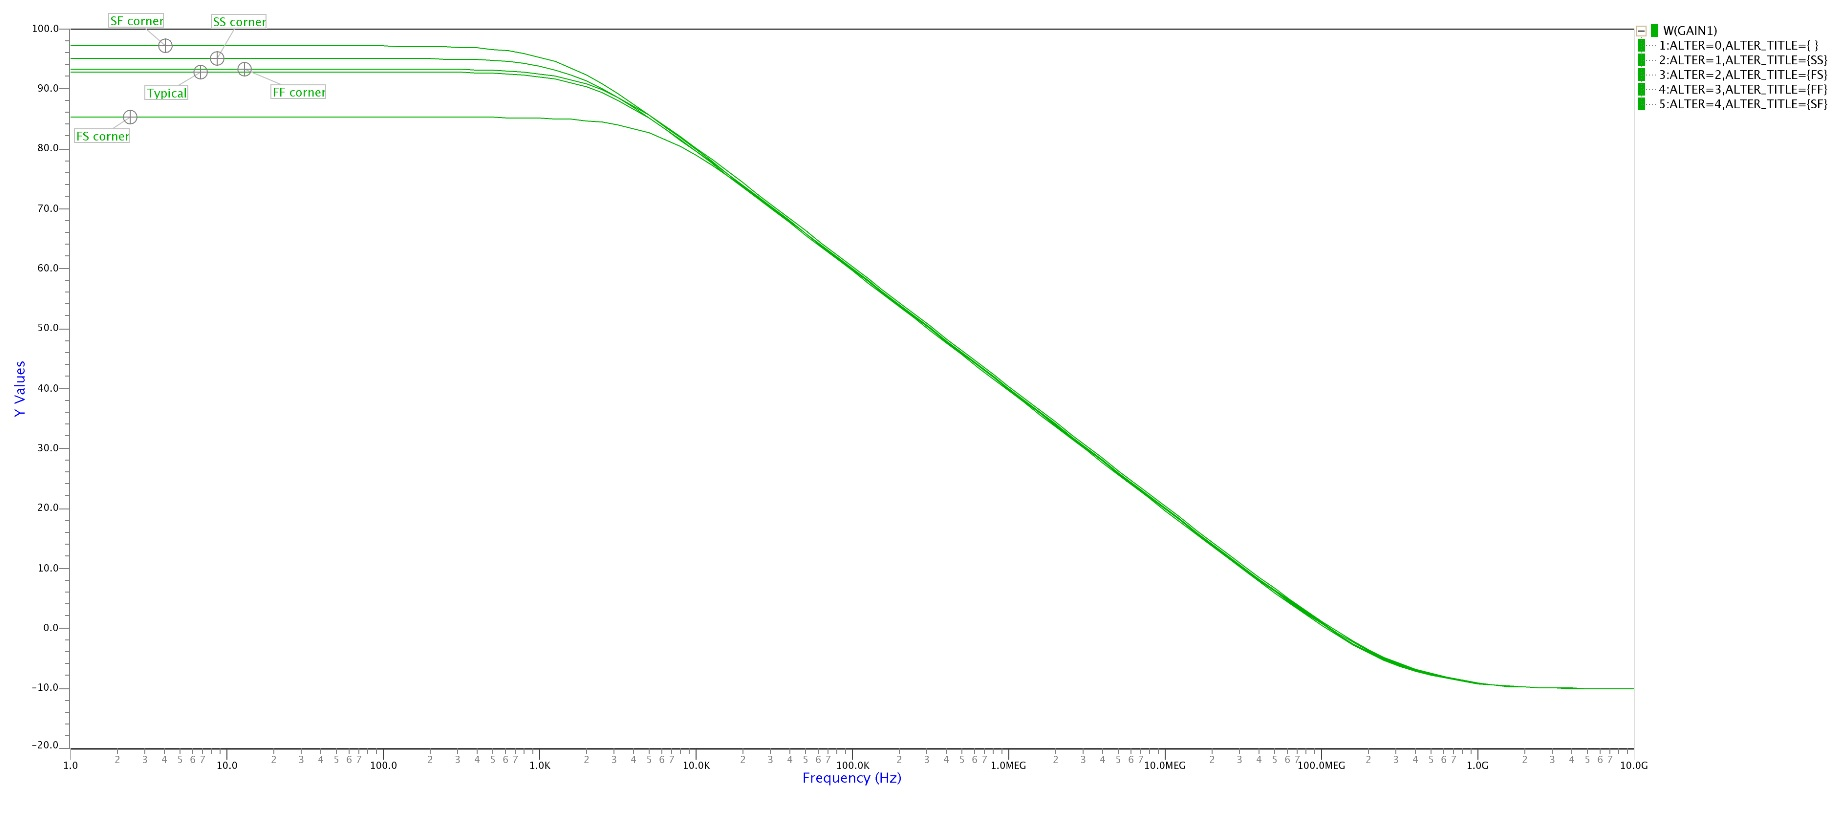
\includegraphics[width=0.8\linewidth]{figures/prakash_fig/opamp_gain_m_rt.JPG}
  \caption{Corner analysis of the op-amp gain, with improved gain booster circuit}
  \label{fig:opamp_gain_m_rt}
\end{figure}

With the modified gain booster circuit, the overall gain of the op-amp at the FS-corner(worst case) is increased from 67dB to 86dB. Analysis of this fix is being done and will be implemented in the layout.  
